\documentclass[bibliography=numbered]{article}
\usepackage[utf8]{inputenc}
\usepackage[a4paper, total={6in, 8in}]{geometry}
\usepackage{graphicx}
\usepackage{parskip}
\usepackage{amsmath}
\usepackage{amsfonts}
\usepackage{hyperref}
\usepackage{multirow}
\usepackage[section]{placeins}
\hypersetup{
    colorlinks=true,
    linkcolor=blue,
    filecolor=white,      
    urlcolor=blue,
    }

\usepackage{biblatex} %Imports biblatex package
\addbibresource{ref.bib} %Import the bibliography file

\usepackage{caption}
\usepackage{subcaption}

\urlstyle{same}

\title{LAMMbert: an automated market maker defined by the Lambert W function}

\author{
  Michael Bentley \\
  \texttt{michael@euler.xyz}}
  
\date{Novermber 2023}

\begin{document}

\maketitle

\section{Introduction}

Two popular automated market makers (AMM) are the constant-sum (CSMM) and constant-product (CPMM) market makers. A simple version of the CSMM is defined by the equation 

\begin{equation}
\label{eq:cs}
    x + y 
    =
    2.
\end{equation}

A simple version of the CPMM is defined by the equation 

\begin{equation}
\label{eq:cp}
    xy 
    = 
    1.
\end{equation}

Our goal is to combine these two functions in such a way as to reveal a relationship between AMMs and the Lambert W function. We begin by multiplying through equation \eqref{eq:cs} by a liquidity concentration parameter $c \geq 0$ to get

\begin{equation}
\label{eq:cs-2}
    c(x + y)
    =
    2c.
\end{equation}

We then take the natural log of both sides of equation \eqref{eq:cp} to get

\begin{equation}
\label{eq:cp-2}
    \ln{xy}
    = 
    0.
\end{equation}

Then adding equations \eqref{eq:cs-2} and \eqref{eq:cp-2} we obtain

\begin{equation}
\label{eq:stable}
    c(x + y) + \ln{xy}
    = 
    2c.
\end{equation}

This equation combines the CSMM and CPMM equations in an interesting way that is similar to StableSwap \cite{egorov2019stableswap}. When $c = 0$ we have a pure CPMM equation, when $c$ grows large it tends towards a pure CSMM equation. 

We now show that equation \eqref{eq:stable} can be solved using the Lambert W function. Exponentiating both sides, and rearranging, we have

\begin{equation}
\label{eq:lambert}
    xe^{cx}
    = 
    \frac{e^{2c-y}}{y}.
\end{equation}

The Lambert W function is defined such that $W(xe^x) = x$. So we can re-write the prior equation by taking $W$ of both sides, to get

\begin{equation}
\label{eq:lambert-2}
    x
    = 
    \frac{1}{c} \cdot W\left( \frac{e^{2-y}}{y} \right).
\end{equation}

Thus, unlike StableSwap, equation \eqref{eq:lambert} can be written in explicit form using the Lambert W function. We call this the LAMMbert AMM. A depiction is shown in Fig. \ref{fig:lambertw}. Equations of this form appear in the solution of linear constant-coefficient delay equations \cite{corless1996lambert}, although it is unclear what, if any, the relationship between those equations and AMMs are. 

Note that there are currently no audited methods to use the Lambert W function on chain, so it is unclear whether or not LAMMbert can be brought to life in a live smart contract today. However, a recent proposal to add such a function to the \href{https://github.com/Vectorized/solady/pull/706}{solady} repository may change this in the near future.

\begin{figure}
    \centering
    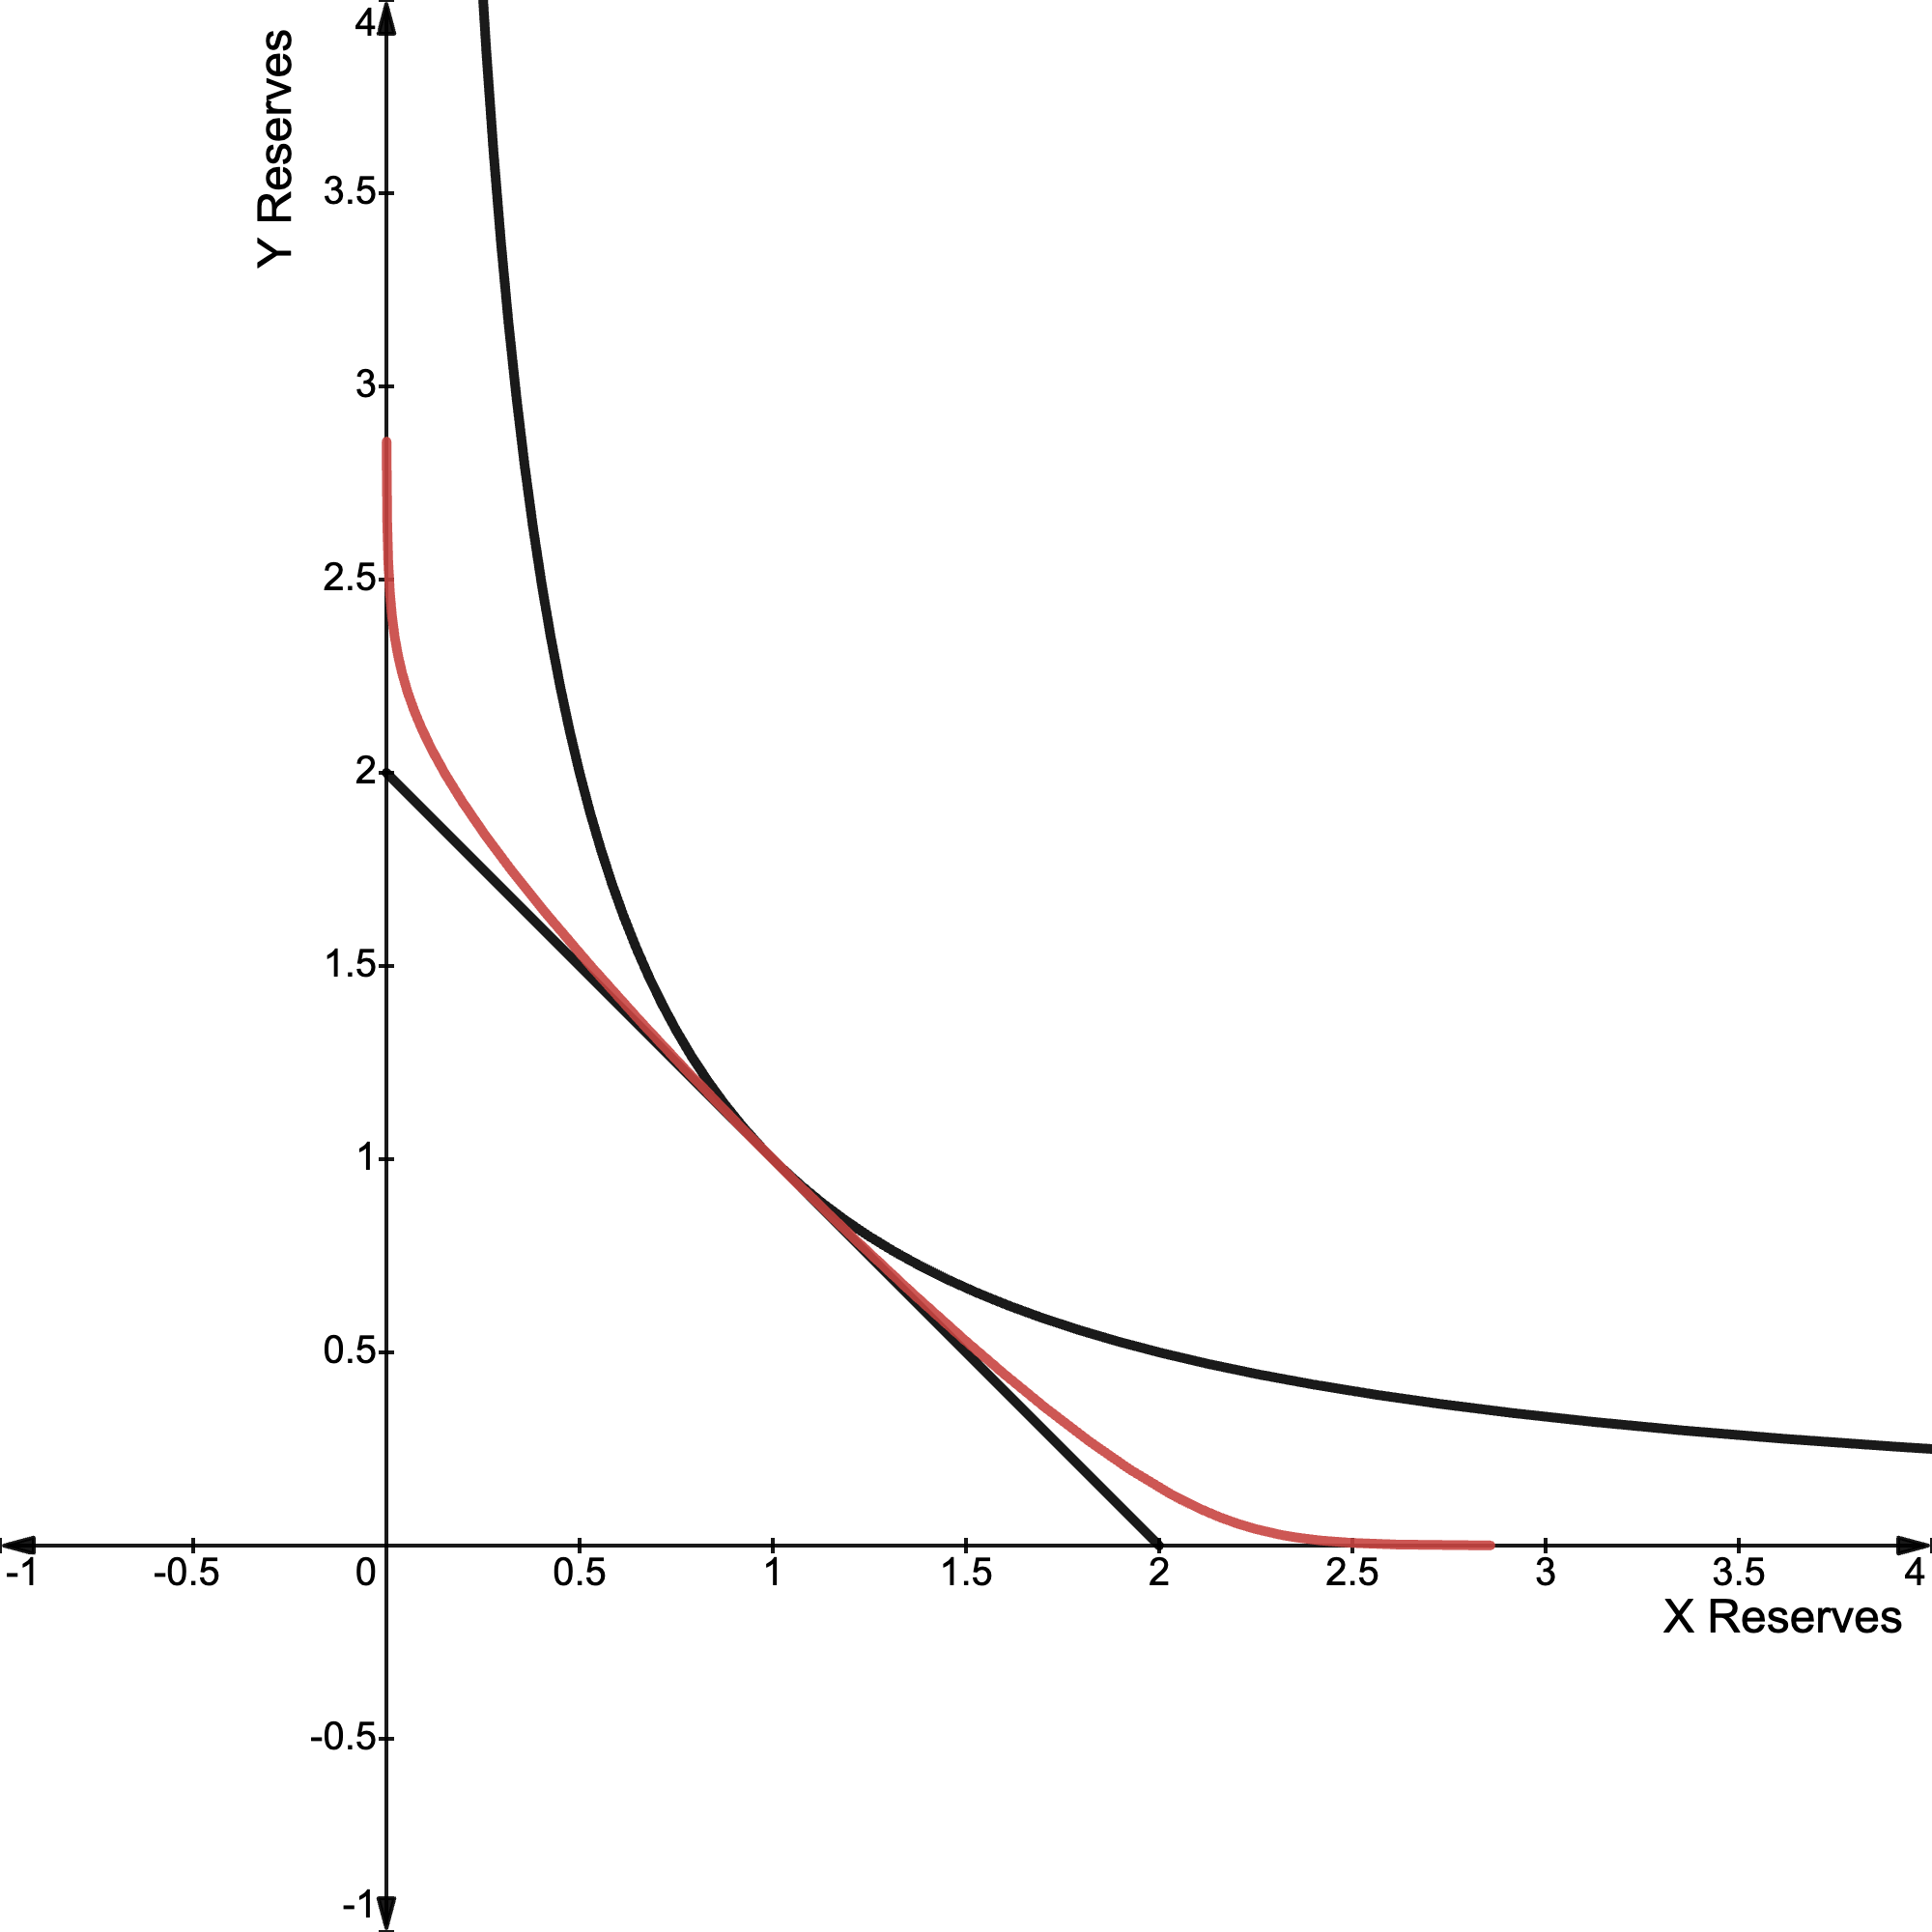
\includegraphics[width=0.5\linewidth]{lambertw.png}
    \caption{\textbf{The LAMMbert automated market maker}. Constant-sum and constant-product market makers can be combined to give an intermediate curve that depends on a concentration parameter. The curve is explicitly defined in terms of the Lambert W function. Desmos link \href{https://www.desmos.com/calculator/9jx4j0rvzm}{here}.}
    \label{fig:lambertw}
\end{figure}

\printbibliography %Prints bibliography

\end{document}

